\section*{Этап 1}

\addcontentsline{toc}{section}{Этап 1}

\subsection*{Описание предметной области}

Существует вселенная, где герои живут уже тысячи лет. Новые герои поставляются корпорацией и имеют разный запас здоровья.\\

Есть пользователи, те инопланетные существа, которые покупают героев и зарабатывают на боях своих героев.\\

Герои деруться нотами из песен, с каждым героем корпорация поставляет в комплекте несколько песен, которые постепенно открываются с растущим опытом героя. Песня может измельчаться на ноты, своеобразные "патроны", которые наносят урон.

\addcontentsline{toc}{subsection}{Описание предметной области}

\subsection*{Описание бизнес процессов}

\addcontentsline{toc}{subsection}{Описание бизнес процессов}

При первом входе в игру дается 1000 золота и 0 опыта.\\
    
Игроки покупают героев. У игроков есть валюта, чтобы платить за героев, у героев есть цена.\\

После покупки героев, игроки выставляют по одному герою на поле битвы. Участие может принимать два игрока и ходят по очереди, тот кто ходит первый определяется рандомом.\\

Перед сражением игрок может выбрать эффект, с которым будет ходить его герой всю битву и песню, которую будет в этой битве исполнять. Эффекты будут следующие: Увеличить своё здоровье, уменьшить здоровье противника, увеличить свой урон, уменьшить урон противника.\\

Герои дерутся между собой, оружием являются ноты, компоненты песен, которые идут в инвентаре с покупными героями. Песни имеют минимальный уровень опыта, который должен иметь герой, чтобы начать их использовать. То есть песни разблокируются постепенно.\\

Чтобы ставить на арену, у нас будет подбор по кол-ву опыта в пределах 100 очков.\\
    
После того, как разыгралось сражение и есть выигравший герой. У всех игроков отнимается 100 золота перераспределяется в пропорциях равных, кол-ву нанесённого урона. \\

Если деньги заканчиваются, игроку необходимо либо купить игровые деньги за валюту, либо открыть лутбокс, который выдаётся каждому игроку раз в день. \\

У нас есть константное значение - кол-во опыта для награждения. В нашем случае это число 10. Мы расчитываем коэффициент, который будет равень модулю разницы опыта игроков, деленный на 10 и прибавляем к нашей константе.

\subsection*{Сущности}

\addcontentsline{toc}{subsection}{Сущности}

\begin{itemize}
\item \textbf{Стержневые сущности}
\begin{enumerate}
    \item Песня(id, имя, порог\_опыта, id\_героя)
    \item Нота(id, имя, урон)
    \item Игрок(id, имя, баланс)
    \item Персонаж(id, опыт, id\_героя, id\_игрока)
    \item Эффект(id, название, цена, цель, здоровье, урон)
    \item Драка(id, время\_начала, время\_конца, id\_локации)
\end{enumerate}

\item \textbf{Ассоциативные сущности}
\begin{enumerate}
    \item Песни\_к\_нотам(id\_песни, id\_ноты)
    \item Участник\_драки(id\_персонажа, id\_драки, id\_эффекта\_в\_драке, id\_используемой\_песни, нанесённый\_урон)
\end{enumerate}

\item \textbf{Характеристические сущности}
\begin{enumerate}
    \item Герой(id, имя, цена, здоровье)
    \item Локация(id, название)
\end{enumerate}
\end{itemize}

\section*{Этап 2}

\addcontentsline{toc}{section}{Этап 2}

\subsection*{Нарисовать ER-диаграмму предметной области}

\addcontentsline{toc}{subsection}{Нарисовать ER-диаграмму предметной области}

\begin{figure}[H]
	\begin{center}
		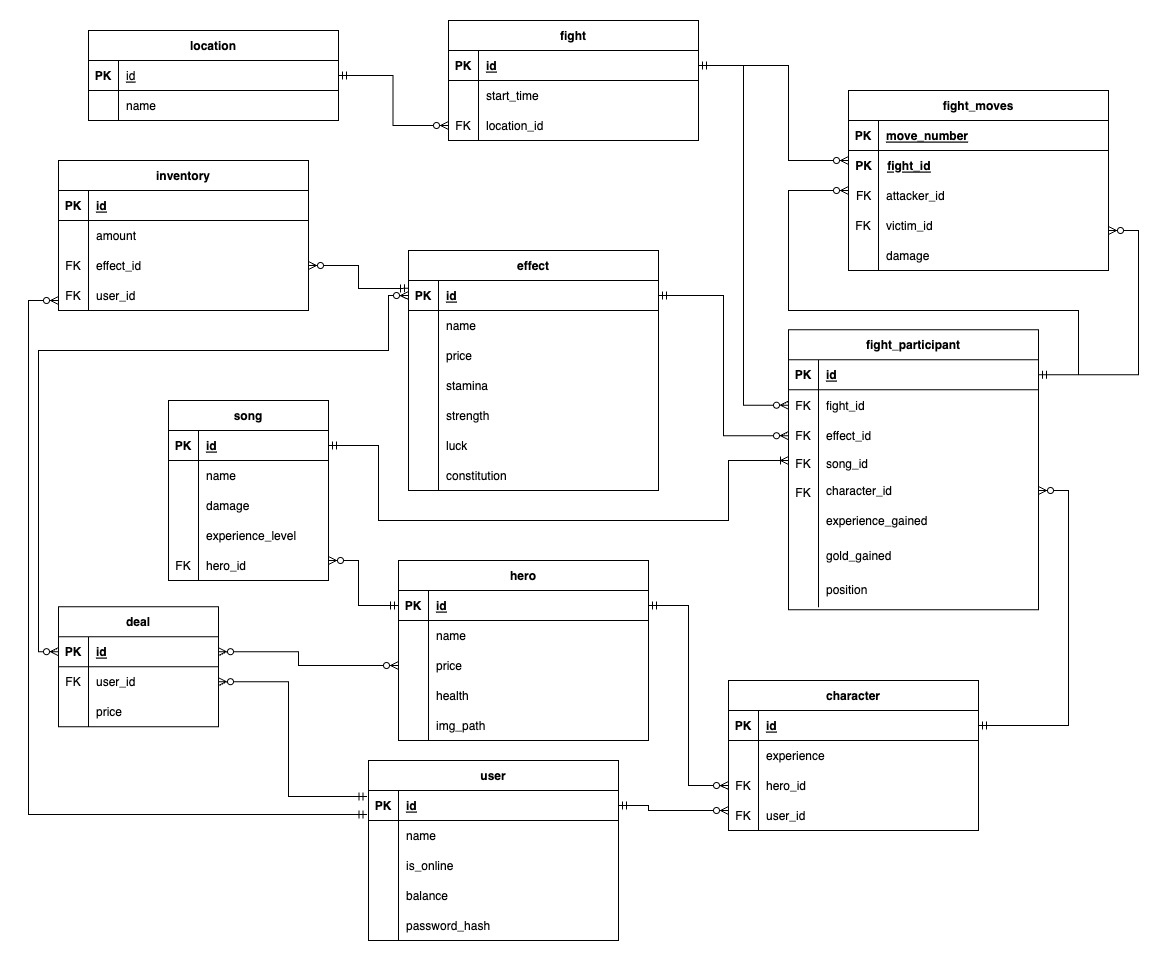
\includegraphics[scale=0.48]{images/ER.jpg}
		\caption{ER-диаграмма предметной области}
	\end{center}
\end{figure}

\subsection*{На основе ER-модели построить даталогическую модель}

\addcontentsline{toc}{subsection}{На основе ER-модели построить даталогическую модель}

\begin{figure}[H]
	\begin{center}
		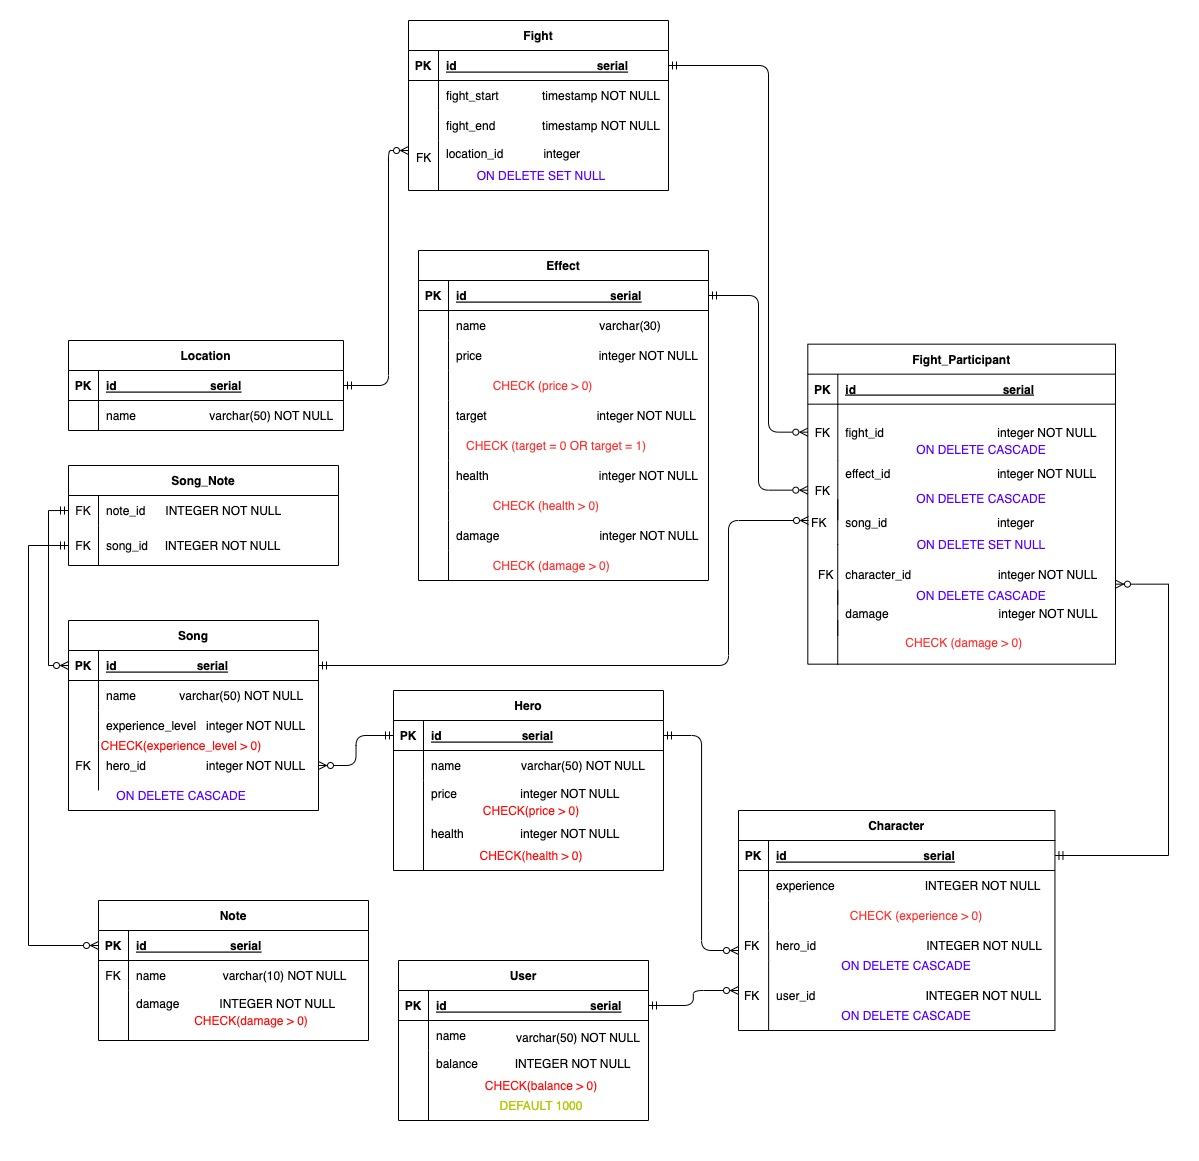
\includegraphics[scale=0.44]{images/Datalogical.jpg}
		\caption{Даталогическая модель}
		\label{pic:pic_name} % название для ссылок внутри кода
	\end{center}
\end{figure}